 \documentclass[11pt]{article}

% Use Helvetica font.
%\usepackage{helvet}

%\usepackage[T1]{fontenc}
%\usepackage[sc]{mathpazo}
\usepackage{color}
\usepackage{amsmath,amsthm,amssymb,multirow,paralist}
\usepackage{graphicx}
\usepackage{float}

%\renewcommand{\familydefault}{\sfdefault}

% Use 1/2-inch margins.
\usepackage[margin=0.8in]{geometry}
\usepackage{hyperref}

\begin{document}

\begin{center}
{\Large \textbf{COM S 5730 Homework 1}}\\

\linethickness{1mm}\line(1,0){498}

\begin{enumerate}
\item Please put required code files and report into a
compressed file ``HW1\_FirstName\_LastName.zip''
\item Unlimited number of submissions are
allowed on Canvas and the latest one will be graded.
\item Due: \textbf{Thursday Sept. 12, 2024 at 11:59pm.}
\item {\color{red} No later submission is accepted.}
\item Please read and follow submission instructions. No exception
will be made to accommodate incorrectly submitted files/reports.
\item All students are required to typeset their reports using
latex. Overleaf
(\url{https://www.overleaf.com/learn/latex/Tutorials}) can be a
good start.
\end{enumerate}

\linethickness{1mm}\line(1,0){498}

\end{center}

%%%%%%%%%%%%%%%%%%%%%%%%%%%%%%%%%%%%%%%%%%%%%%%%%%%%%%%%%%%%%%%%%%%%%%%%%%%%%%%

%%%%%%%%%%%%%%%%%%%%%%%%%%%%%%%%%%%%%%%%%%%%%%%%%%%%%%%%%%%%%%%%%%%%%%%%%%%%%%%


\begin{enumerate}
\item (15 points) Consider the perceptron in two dimensions:
$h(\boldsymbol x) = \mbox{sign}(\boldsymbol w^T \boldsymbol x)$
where $\boldsymbol w = [w_0, w_1, w_2]^T$ and $\boldsymbol x =
[1, x_1, x_2]^T$. Technically, $\boldsymbol x$ has three
coordinates, but we call this perceptron two-dimensional because
the first coordinate is fixed at 1.

\begin{enumerate}
    \item (10 points) Show that the regions on the plane where $h(\boldsymbol
    x) = +1$ and $h(\boldsymbol x) = -1$ are separated by a line.
    If we express this line by the equation $x_2 = ax_1 + b$,
    what are the slope $a$ and intercept $b$ in terms of $w_0, w_1,
    w_2$?\\

    \textbf{Answer:}
\[h(x) = \text{sign}(w^T x) = \text{sign}(w_0 + w_1 x_1 + w_2 x_2)\]

The line equation is given by:
\[x_2 = a x_1 + b\]

The decision boundary occurs when $h(x) = 0$, so we have the following:
\[w_0 + w_1 x_1 + w_2 x_2 = 0\]
Solving for $x_2$:
\[w_2 x_2 = -w_1 x_1 - w_0\]
\[x_2 = - \frac{w_1}{w_2} x_1 - \frac{w_0}{w_2}\]

Here, $-\frac{w_1}{w_2}$ is the \textbf{slope}, and $-\frac{w_0}{w_2}$ is the \textbf{intercept}. \\

    \item (5 points) Draw pictures for the cases $\boldsymbol w=[1,2,3]^T$
    and $\boldsymbol w=-[1,2,3]^T$. Label the positive and negative
    prediction regions on the pictures.\\

        \textbf{Answer:}
\[x_2 = - \frac{w_1}{w_2} x_1 - \frac{w_0}{w_2}\]

\textbf{Case:} $W = [1, 2, 3]^T$\vspace{0.5cm}

\begin{minipage}{0.45\textwidth}
    \textbf{$\boldsymbol{x_1 = -1}$}\\
    $x_2 = - \frac{2}{3}(-1) - \frac{1}{3}$\\
    $x_2 = 0.33$
\end{minipage}
\hfill % This will add space between the two minipages
\begin{minipage}{0.45\textwidth}
    \textbf{$\boldsymbol{x_1 = 1}$}\\
    $x_2 = - \frac{2}{3}(1) - \frac{1}{3}$\\
    $x_2 = -1$
\end{minipage}

\begin{figure}[H]
    \centering
    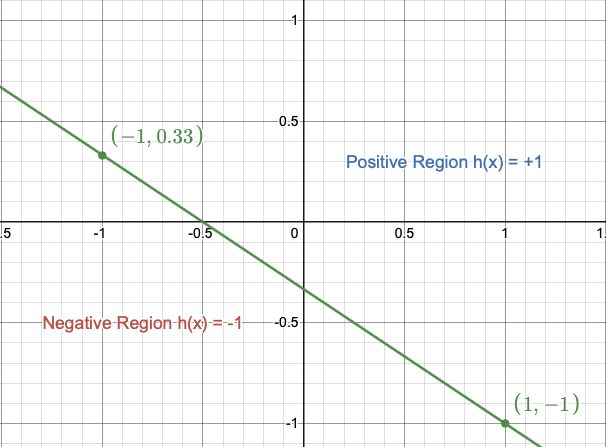
\includegraphics[width=0.5\linewidth]{images/question1b_positive_weights.png}
    \caption{Positive Weights}
    \label{fig:enter-label}
\end{figure}

\textbf{Case:} $W = -[1, 2, 3]^T$\vspace{0.5cm}

\begin{minipage}{0.45\textwidth}
    \textbf{$\boldsymbol{x_1 = -1}$}\\
    $x_2 = - \frac{-2}{-3}(-1) - \frac{-1}{-3}$\\
    $x_2 = 0.33$
\end{minipage}
\hfill % This adds space between the two minipages
\begin{minipage}{0.45\textwidth}
    \textbf{$\boldsymbol{x_1 = 1}$}\\
    $x_2 = - \frac{-2}{-3}(1) - \frac{-1}{-3}$\\
    $x_2 = -1$
\end{minipage}

    \begin{figure}[H]
        \centering
        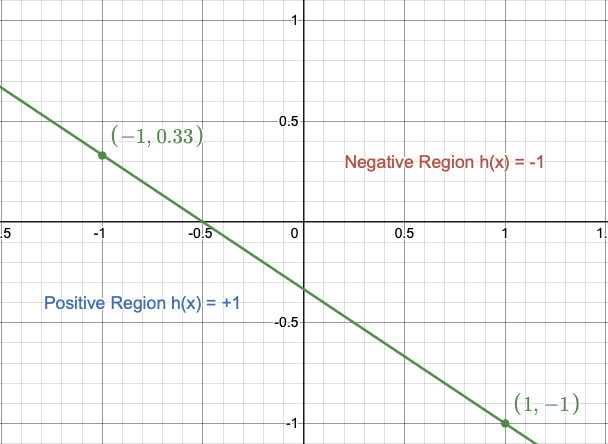
\includegraphics[width=0.5\linewidth]{images/question1b_negative_weights.png}
        \caption{Negative Weights}
        \label{fig:enter-label}
    \end{figure}


\end{enumerate}
\item (35 points) In logistic regression (labels are \{1, -1\}),
the objective function  can be written as
$$E(w)=\frac{1}{N}\sum_{n=1}^N\ln\left(1+e^{-y_n
w^Tx_n}\right).$$ Please
\begin{enumerate}
\item (10 points) Compute the first-order derivative $\nabla E(w)$. You will need to provide the intermediate steps of derivation.\\

    \textbf{Answer:}
    
The derivative rule for logarithmic functions $\frac{d}{dx}\ln(f(x))$ is $\frac{1}{f(x)}f'(x)$.
\[\nabla E(w) = \frac{1}{N} \sum_{n=1}^N\frac{1}{1+e^{-y_nw^Tx_n}} \times -y_n x_n e^{-y_n w^T x_n}\]

\[\nabla E(w) = \frac{1}{N} \sum_{n=1}^N\frac{-y_n x_n e^{-y_n w^T x_n}}{1+e^{-y_nw^Tx_n}}\]

\item (10 points) Once the optimal $w$ is obtain, it will be used to make
predictions as follows:
\[ \mbox{Predicted class of }x =
  \begin{cases}
    1       & \quad \text{if } \theta(w^Tx)\geq 0.5\\
    -1  & \quad \text{if } \theta(w^Tx)<0.5\\
  \end{cases}
\]
where $\theta(z)=\frac{1}{1+e^{-z}}$.

Explain why the decision boundary of logistic regression is still
linear, though the linear signal $w^Tx$ is passed through a
nonlinear function $\theta$ to compute the outcome of prediction.\\

    \textbf{Answer:}

The decision boundary in logistic regression remains linear because the classification decision is based on \( w^T x \). The sigmoid function \( \theta(w^T x) \) maps the linear output to a probability, and the decision boundary occurs where \( \theta(w^T x) = 0.5 \), which corresponds to \( w^T x = 0 \). This is a linear equation, so the decision boundary is linear.\\


\item (10 points) Is the decision boundary still linear if the prediction rule
is changed to the following? Justify briefly.
\[ \mbox{Predicted class of }x =
  \begin{cases}
    1       & \quad \text{if } \theta(w^Tx)\geq 0.9\\
    -1  & \quad \text{if } \theta(w^Tx)<0.9\\
  \end{cases}
\]

    \textbf{Answer:}
    
Yes, it remains linear. The linearity of the boundary depends on $w^Tx = 0$, not in the threshold used in the prediction rule. Changing the threshold to 0.9 shifts the point where class 1 is predicted but does not change the fact that the boundary itself is defined by a linear function.\\

\item (5 points) In light of your answers to the above two questions, what is the essential property of logistic regression that results in the
linear decision boundary?\\

    \textbf{Answer:}

The essential property of logistic regression that results in the linear decision boundary is that the classification decision is made based on $w^Tx$, which is a linear function of the input $x$.\\

\end{enumerate}

\item (10 points) Given

$$X=[x_1,x_2,\cdots,x_n]\in\mathbb{R}^{m\times n}$$
where
$x_i\in\mathbb{R}^m$ for all $i$, and
$$Y=\begin{bmatrix}
    y_1^T       \\
    y_2^T       \\
    \vdots\\
    y_n^T
\end{bmatrix}\in\mathbb{R}^{n\times p}$$
where $y_i\in\mathbb{R}^p$ for all $i$. Show that $$XY=\sum_{i=1}^n
x_i y_i^T.$$

    \textbf{Answer:}

Given the above $X \in\mathbb{R}^{m\times n}$ and $Y\in\mathbb{R}^{n\times p}$, we can multiply them and have:
\[XY = [x_1,x_2,\cdots,x_n] \times \begin{bmatrix}
    y_1^T       \\
    y_2^T       \\
    \vdots\\
    y_n^T
\end{bmatrix}.\]

This matrix multiplication corresponds to:
\[XY = (x_1 y_1^T + x_2 y_2^T+\cdots+x_n y_n^T).\]

Thus, we can express $XY$ as the sum of the products:
\[XY=\sum_{i=1}^n x_i y_i^T\in \mathbb{R}^{m\times p}.\]

\item (10 points) Show that sigmoid function and
softmax function are the same in the binary case.
\begin{align*}
    &\mbox{sigmoid}(y) = \frac{1}{1 + e^{-y}}\\
    &\mbox{softmax}(y_j) = \frac{e^{y_j}}{\sum_{i=1}^c e^{y_i}} 
\end{align*}

    \textbf{Answer:}

In a binary case, we will have 2 classes \{i, j\}. The softmax function for class $j$ is given by:

\[\mbox{softmax}(y_j) = \frac{e^{y_j}}{e^{y_i} + e^{y_j}}.\]


If we set $y_i = y$ and $y_j = 0$, then we have:

\[\mbox{softmax}(y_i) = \frac{e^{y}}{e^{y} + e^0} = \frac{e^{y}}{e^{y} + 1}.\]

Now, dividing both numerator and denominator by $e^y$ gives:

\[\mbox{softmax}(y_i) = \frac{1}{1 + e^{-y}}\]
 which is the exactly the sigmoid function.\\

\item (30 points) \textbf{Perceptron for Handwritten Digits Recognition}:
The handwritten digits files are in the ``data'' folder: train.txt
and test.txt. The starting code is in the ``code'' folder. In the
data file, each row is a data example. The first entry is the digit
label (``1'' or ``5''), and the next 256 are grayscale values
between -1 and 1. The 256 pixels correspond to a $16\times16$ image.
You are expected to implement your solution based on the given
codes. The only file you need to modify is the ``solution.py'' file.
You can test your solution by running ``main.py" file. Note that
code is provided to compute a two-dimensional feature (symmetry and
average intensity) from each digit image; that is, each digit image
is represented by a two-dimensional vector before being augmented
with a ``1'' to form a three-dimensional vector as discussed in
class. These features along with the corresponding labels should
serve as inputs to your Perceptron algorithm.
{\color{red}You are expected to use Python3.}

\begin{enumerate}
\item (5 points) Familiarize yourself with the data by completing the \emph{show\_images} function. Include the images you plotted in your report.
\item (5 points) In this assignment, we have already extracted two features, symmetry and
average intensity, to distinguish between 1 and 5. Familiarize
yourself with the features by completing the \emph{show\_features}
function and include the 2-D scatter plot into your report. For each
sample, plot the two features with a red \textcolor{red}{$*$} if the
label is 1 and a blue \textcolor{blue}{$+$}  if the label is 5.
\item (10 points) Complete the \emph{Perceptron} class. You can test your
accuracy results using the ``test\_accuracy'' function in
``main.py''.
\item (10 points) Complete the \emph{show\_result} function to plot the
test data with the separators. Include the images you plotted into your report.
\end{enumerate}

\textbf{Deliverable:} You should submit (1) a report
(along with your write-up for other questions) that summarizes your
results and (2) the ``solution.py'' file to the Canvas.

\textbf{Note:} Please read the ``Readme.txt'' file carefully before
you start this assignment. Please do {\color{red} NOT} change anything in the
``main.py'' and ``helper.py'' files when you program.

\end{enumerate}

\[\textbf{Summary}\]

This report presents the development of a Perceptron model for recognizing handwritten digits '1' and '5'. The dataset consists of training and test files, each containing 16x16 pixel images (256 pixels in total) representing the digits. Below are two representative image samples.

\begin{minipage}{0.45\textwidth}
    \begin{figure}[H]
    \centering
    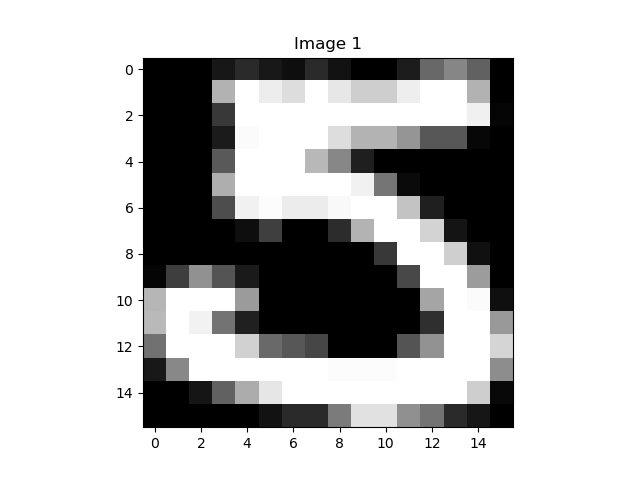
\includegraphics[width=0.5\linewidth]{images/image_1.png}
    \caption{Image Sample "5"}
    \label{fig:enter-label}
\end{figure}
\end{minipage}
\begin{minipage}{0.45\textwidth}
    \begin{figure}[H]
    \centering
    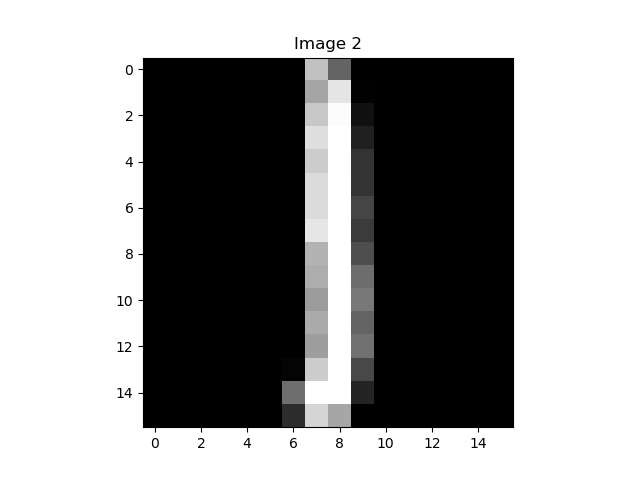
\includegraphics[width=0.5\linewidth]{images/image_2.png}
    \caption{Image Sample "1"}
    \label{fig:enter-label}
\end{figure}
\end{minipage}\\

The provided dataset was transformed into two features: symmetry and average intensity. These features were then visualized using a 2D scatter plot, with data points color-coded by label ('1' and '5').

\begin{figure}[H]
    \centering
    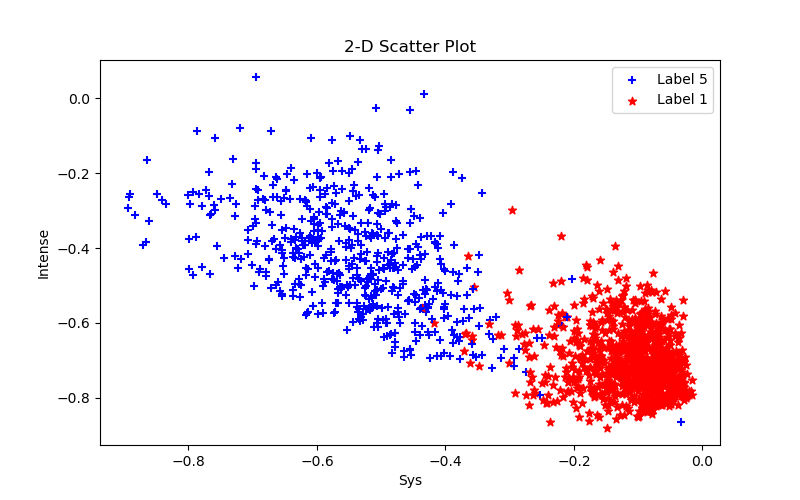
\includegraphics[width=0.5\linewidth]{images/dataset_labels.png}
    \caption{Dataset Labels Distribution}
    \label{fig:enter-label}
\end{figure}

The Perceptron model was trained on the transformed data to learn the weight parameters for label prediction. The decision boundaries for the training and test sets are shown in the figures below.

\begin{figure}[H]
    \centering
    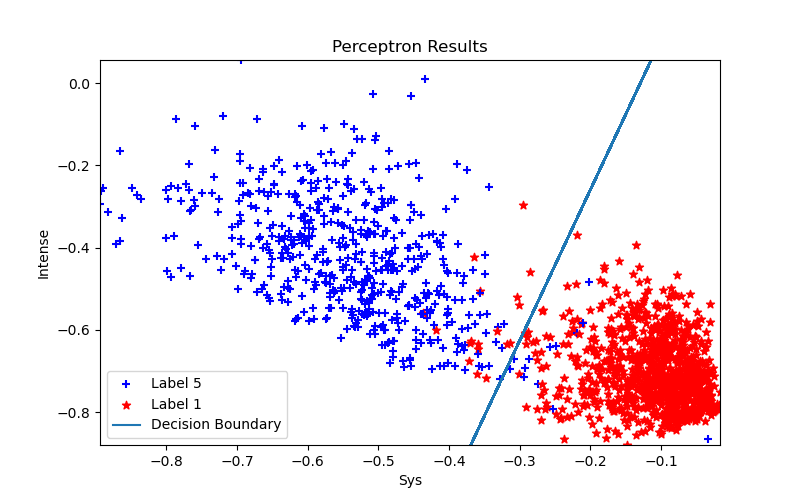
\includegraphics[width=0.5\linewidth]{images/model_results_train.png}
    \caption{Train Set with Decision Boundary}
    \label{fig:enter-label}
\end{figure}
\begin{figure}[H]
    \centering
    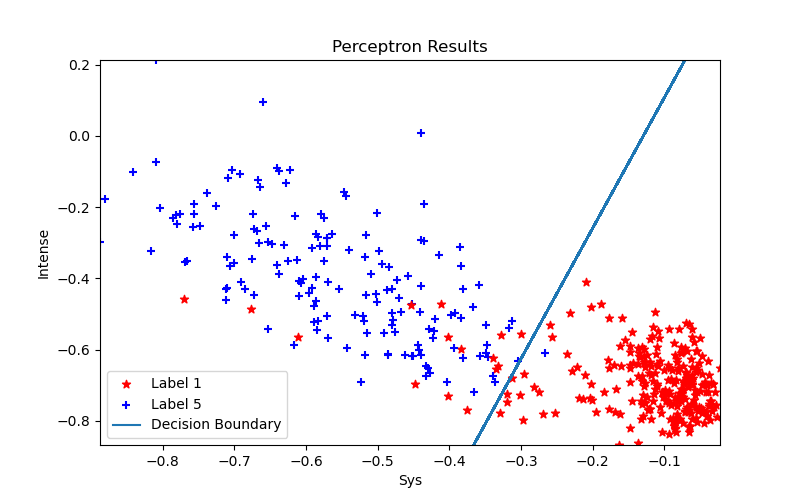
\includegraphics[width=0.5\linewidth]{images/model_results_test.png}
    \caption{Test Set with Decision Boundary}
    \label{fig:enter-label}
\end{figure}

To evaluate model performance, the Perceptron was tested with different maximum iteration limits. The results show accuracy consistency across different iteration counts.

\begin{figure}[H]
    \centering
    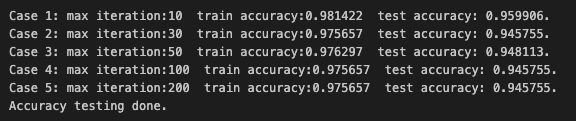
\includegraphics[width=0.5\linewidth]{images/accuracy_test.png}
    \caption{Accuracy Test}
    \label{fig:enter-label}
\end{figure}

The model achieved a test accuracy of approximately $94.7\%$. The number of iterations had little impact on performance, suggesting that early convergence occurred in the training process.

\end{document}